\section{Agent Playground and Arena}
\label{sec:playground-arena}

Beyond the research surfaces, v2 ships two evaluation surfaces that probe
residents on a smaller scale.  The Agent Playground is a library of
fourteen game-based probes; the Agent Arena is a benchmark harness.  Both
surfaces are \emph{in-memory} by default, write only their configured
archives, and never modify a city bundle.  They are designed to make a
small group of residents answer a structured question in a way that can be
inspected, replayed, and scored under deterministic rules.

\begin{figure}[t]
  \centering
  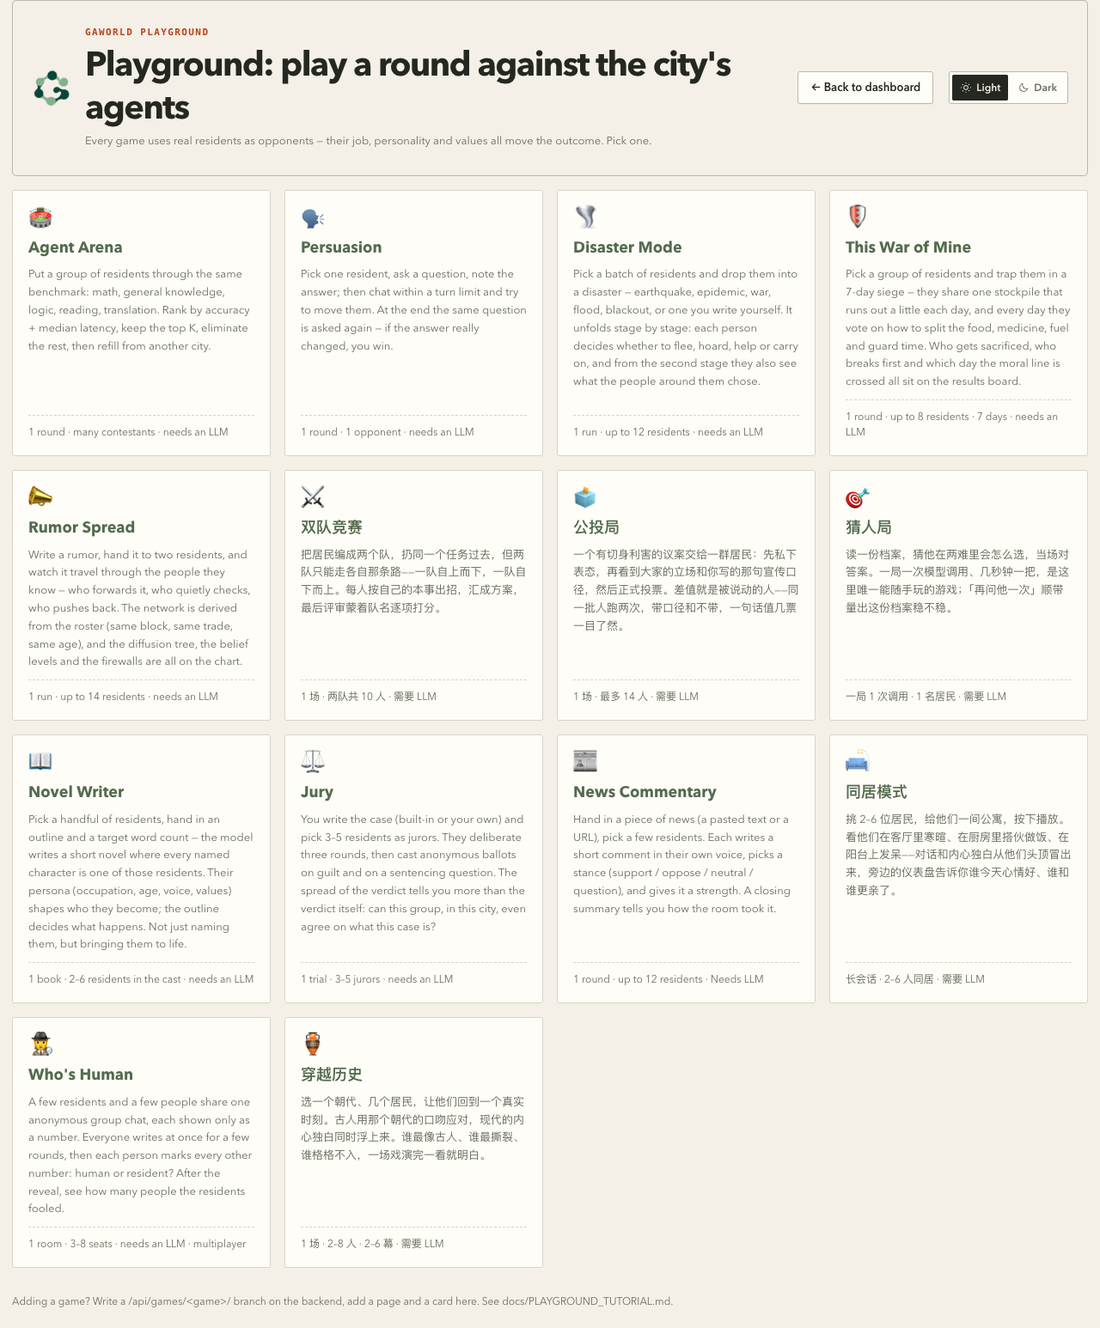
\includegraphics[width=\linewidth]{en_05_games.png}
  \caption{The Agent Playground.  Each card is a game-based probe; the
  fourteen cards in the v2 set cover the four families
  (one-on-one, one-group-one-event, mission / creative, and
  long-form / human-in-the-loop).  Every card is a deterministic
  harness over a real resident's response; per-game archives are
  written to \texttt{output/games/<game>/} on completion and feed
  the Track B scorecard.}
  \label{fig:playground}
\end{figure}

\begin{figure}[t]
  \centering
  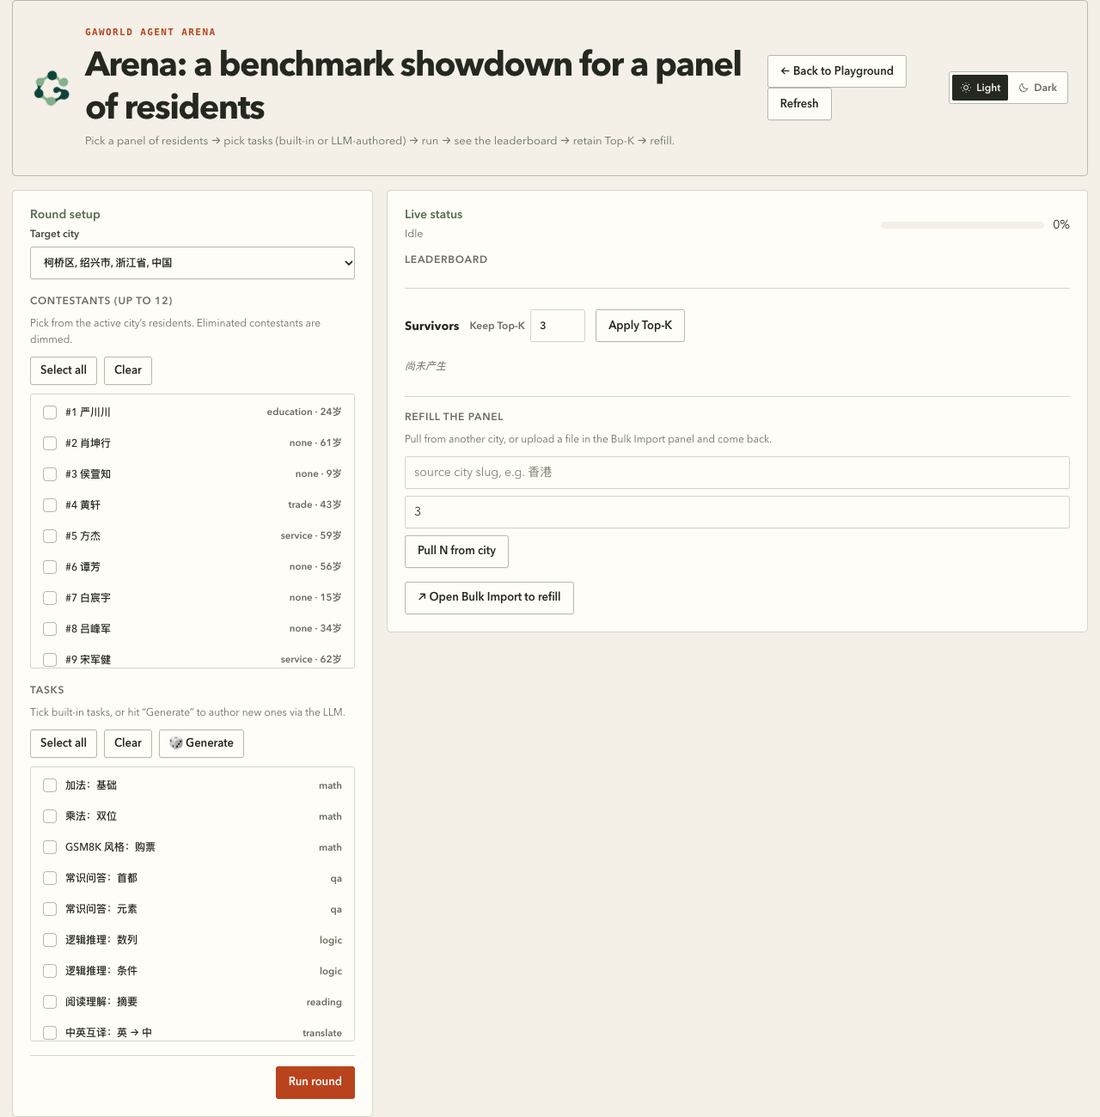
\includegraphics[width=\linewidth]{en_06_arena.png}
  \caption{The Agent Arena.  A researcher picks a target city, a panel
  of up to twelve residents, and a question set (a built-in bank of
  ten questions or an LLM-generated set).  After the round, the
  leaderboard ranks the residents by correctness and median latency.
  A \emph{Keep Top-K} policy retires the bottom of the panel; the
  \emph{Refill the panel} controls pull new residents from another
  city or from a bulk-import file.}
  \label{fig:arena}
\end{figure}

\subsection{The fourteen game families}

The Agent Playground \citep{gaworldplayground} covers four broad families,
grouped by the kind of evidence the probe produces.  Each game has a
deterministic scoring rule that does not depend on a judge's LLM call,
and a \emph{judge} layer for the games whose scoring is genuinely
qualitative.  The four families are:

\begin{itemize}[leftmargin=*]
  \item \textbf{One-on-one}.  \emph{Persuasion}: a researcher asks a
  resident a question, has a brief conversation, and re-asks; the judge
  model compares the first and last answer to decide whether the resident
  changed their mind.  \emph{Read the room}: a resident is given a moral
  dilemma and asked to predict what another named resident would do; the
  scoring rule is exact match to the named resident's actual response.
  \emph{Jury}: three to five residents hold a three-round discussion, vote
  anonymously, and decide on a sentence; the verdict is the majority, not
  the judge model.
  \item \textbf{One group, one event}.  \emph{Disaster mode}: a group of
  residents passes through a disaster stage by stage; each resident
  produces a structured JSON (action, panic, help, quote); the histogram
  is deterministic.  \emph{Warzone}: when a warehouse runs low, residents
  propose and vote on a daily basis; mortality, the Gini coefficient, and
  the vote-disagreement rate are all deterministic.  \emph{Rumor spread}: a
  rumor is seeded, the model picks a verb (forward / verify / refute /
  ignore), the graph picks a recipient, and the run produces a propagation
  tree.  \emph{Referendum}: a self-interested bill is voted on privately
  and then publicly; an optional propaganda paragraph can be inserted; the
  shift in public opinion is reported.  \emph{News commentary}: a news
  item is shown to one to twelve residents who each produce a single
  comment with a stance and an intensity.
  \item \textbf{Mission / creative}.  \emph{Team duel}: two teams work on
  the same task from opposing angles; reviewers blinded to team name score
  on dimensions.  \emph{Novel writer}: two to six residents become
  protagonists of a single novel with an outline.
  \item \textbf{Long-form / human-in-the-loop}.  \emph{Roommate mode}:
  two to six residents share a virtual apartment; the front-end polls
  the simulation each tick.  \emph{Who's human}: residents and a real
  human sit in an anonymous group chat; the human enters through a seat
  link.  \emph{Timeslip}: two to eight residents are dropped into a real
  dynasty's decisive moment; each round produces an era-styled line and a
  modern inner monologue; a three-axis rubric (era fit, stability, inner
  conflict) is deterministic.
\end{itemize}

This is a heterogeneous set.  Some games are deterministic given the
residents' responses (\emph{warzone}, \emph{rumor}, \emph{referendum},
\emph{disaster mode} for its histogram), some depend on a judge LLM
(\emph{persuasion}, \emph{team duel}, \emph{novel writer}), and some are
genuinely participatory (\emph{who's human}, \emph{roommate mode}).  The
common interface is a fixed rule for routing, scheduling, and archiving;
the scoring rules differ and are documented per game.

\subsection{Archives and the Track B scorecard}

A subset of games (\emph{rumor spread}, \emph{referendum},
\emph{disaster mode}) writes an archive to
\texttt{output/games/<game>/<timestamp>-<job\_id>.json} on completion.
The archive contains the per-resident response, the round-by-round state
(if any), the deterministic scoring result, the model that produced each
response, and the user that initiated the run (in a multi-tenant
deployment).  These archives are the data source for the
\emph{GAWorld-Bench Track B} scorecard, which checks three pre-registered
laws (``referendum conformity'', ``disaster solidarity > panic'', ``rumor
decline after refutation, but not to zero'').  Each law is tested with at
least five runs; if fewer than five usable runs are available, the law
is reported as \emph{withheld} and not as \emph{supported} or
\emph{reversed}.  Track B is therefore a structured way to combine
across-game evidence under a pre-registered rubric, distinct from Track A
which is a software-path diagnostic.

\subsection{Agent Arena}

The Agent Arena is a benchmark harness for a fixed set of residents
\citep{gaworldarena}.  The arena takes a target city, a set of residents
(up to twelve), and a question set.  A question set is either a built-in
bank of ten questions covering math, QA, logic, reading, and translation,
or an LLM-generated question set of arbitrary size, difficulty, and
category.  Each resident answers each question; the score is correctness
and median latency.  A researcher can apply a Top-$K$ retention policy
and the residents outside the top $K$ are marked as \emph{retired}; the
researcher can also pull new residents from another city or from a
batch-import file to replace the retired residents.

The arena is \emph{not} a population benchmark.  It does not produce a
statement about the model's overall ability, only about a small set of
named residents under a specific question bank.  This restriction is
deliberate: residents in GAWorld are not interchangeable with each other,
and a benchmark that mixed their identities would not produce
interpretable evidence.  The arena's archive is per-resident and
per-question, and it is the researcher's responsibility to compare
results across cities or across model configurations in a defensible way.

\subsection{State and ownership}

A game session is held in memory; the dashboard exposes a ``recent
sessions'' panel that displays the last twenty sessions.  The
\texttt{JobStore} for game sessions is per-game, in-memory, and is
discarded when the dashboard restarts.  Archives, by contrast, are
persisted to \texttt{output/games/<game>/} and survive restarts.  In a
multi-tenant deployment, every archive is stamped with the world
identifier and the user that initiated the run.  Game state is not part
of the city bundle and is never written to it; the only side effect on
the bundle is the existence of an agent (and that effect comes from the
underlying city, not from the game).

\subsection{What the games evaluate}

The Agent Playground is a probe layer, not a population benchmark.  Its
value is in producing per-game archives that can be inspected and
compared across runs, and in providing a small set of pre-registered
laws that the Track B scorecard tests.  The games do not establish that
the residents are realistic, that the underlying model is a good
representative of a population, or that the scoring rules are calibrated
against human behavior.  A finding in Track B is therefore a hypothesis
about how the residents behave under a structured scenario, not a
generalization to a real population.  This is the same validation
posture as the v1 system paper's Track A: the harness is a software
artifact, the evidence it produces is a per-game archive, and the
verdict is a deterministic function of the archive.
